\documentclass[10pt]{beamer}

\usetheme[progressbar=frametitle]{metropolis}
\usepackage{appendixnumberbeamer}

\usepackage{booktabs}
\usepackage[scale=2]{ccicons}

\usepackage{pgfplots}
\usepgfplotslibrary{dateplot}

\usepackage{braket} %ket vectors
\usepackage[font=footnotesize,labelfont=bf]{caption}
\usepackage{parskip} %automatic paragraphing
\usepackage{color}
\usepackage{dsfont}%identity operator
\usepackage{mathrsfs}
\usepackage{xspace}
\usepackage{amsmath} %for gathering equations
\usepackage{siunitx} %for SI units
\usepackage{pgfplots} %for plotting
\usepackage{filecontents} %for data loading
\begin{filecontents}{datax.dat}
0.06941, 28, 0.44096, 30, 0.15165, 25
0.04389, 146, 0.32707, 132,0.10722, 109
0.02823, 3622, 0.08416, 3478, 0.02086, 2997
0.01008, 17838, 0.005179, 17566, 0.01494, 14721
0.00165, 89130,0.0015799, 88216, 0.003327, 74009
%0.00156, 444646, 0.0015601, 439060, 0.001578, 370813
%previous 3rd row: 0.04951, 728, 0.224107, 642, 0.020864, 601

\end{filecontents}

\usepackage[cal=zapfc,calscaled=.96]{mathalfa}

\newcommand{\themename}{\textbf{\textsc{metropolis}}\xspace}

\title{Putting quantum machine learning algorithms to the test}
\subtitle{4th QIPCC conference, 2016 \newline Cape Town, South Africa}
% \date{\today}
\date{}
\author{Mark Fingerhuth}
\institute{Maastricht University, The Netherlands \newline Thesis work at Centre for Quantum Technology, UKZN, South Africa }
% \titlegraphic{\hfill
\includegraphics[height=1.5cm]{logo.pdf}}

\begin{document}

\maketitle

\begin{frame}{Table of contents}
  \setbeamertemplate{section in toc}[sections numbered]
  \tableofcontents[hideallsubsections]
\end{frame}

\section{Introduction}

{
\setbeamertemplate{frame footer}{\tiny{\textsuperscript{1}Reprinted from Wikipedia, n.d., Retrieved September 7, 2016, from \url{https://en.wikipedia.org/wiki/Bloch_Sphere}. Copyright 2012 by Glosser.ca. Reprinted with permission.}}
\begin{frame}[fragile]{Quantum Computing \& Qubits}

\begin{minipage}[c]{.5\textwidth}
		%\centering
		\hspace{2mm}
       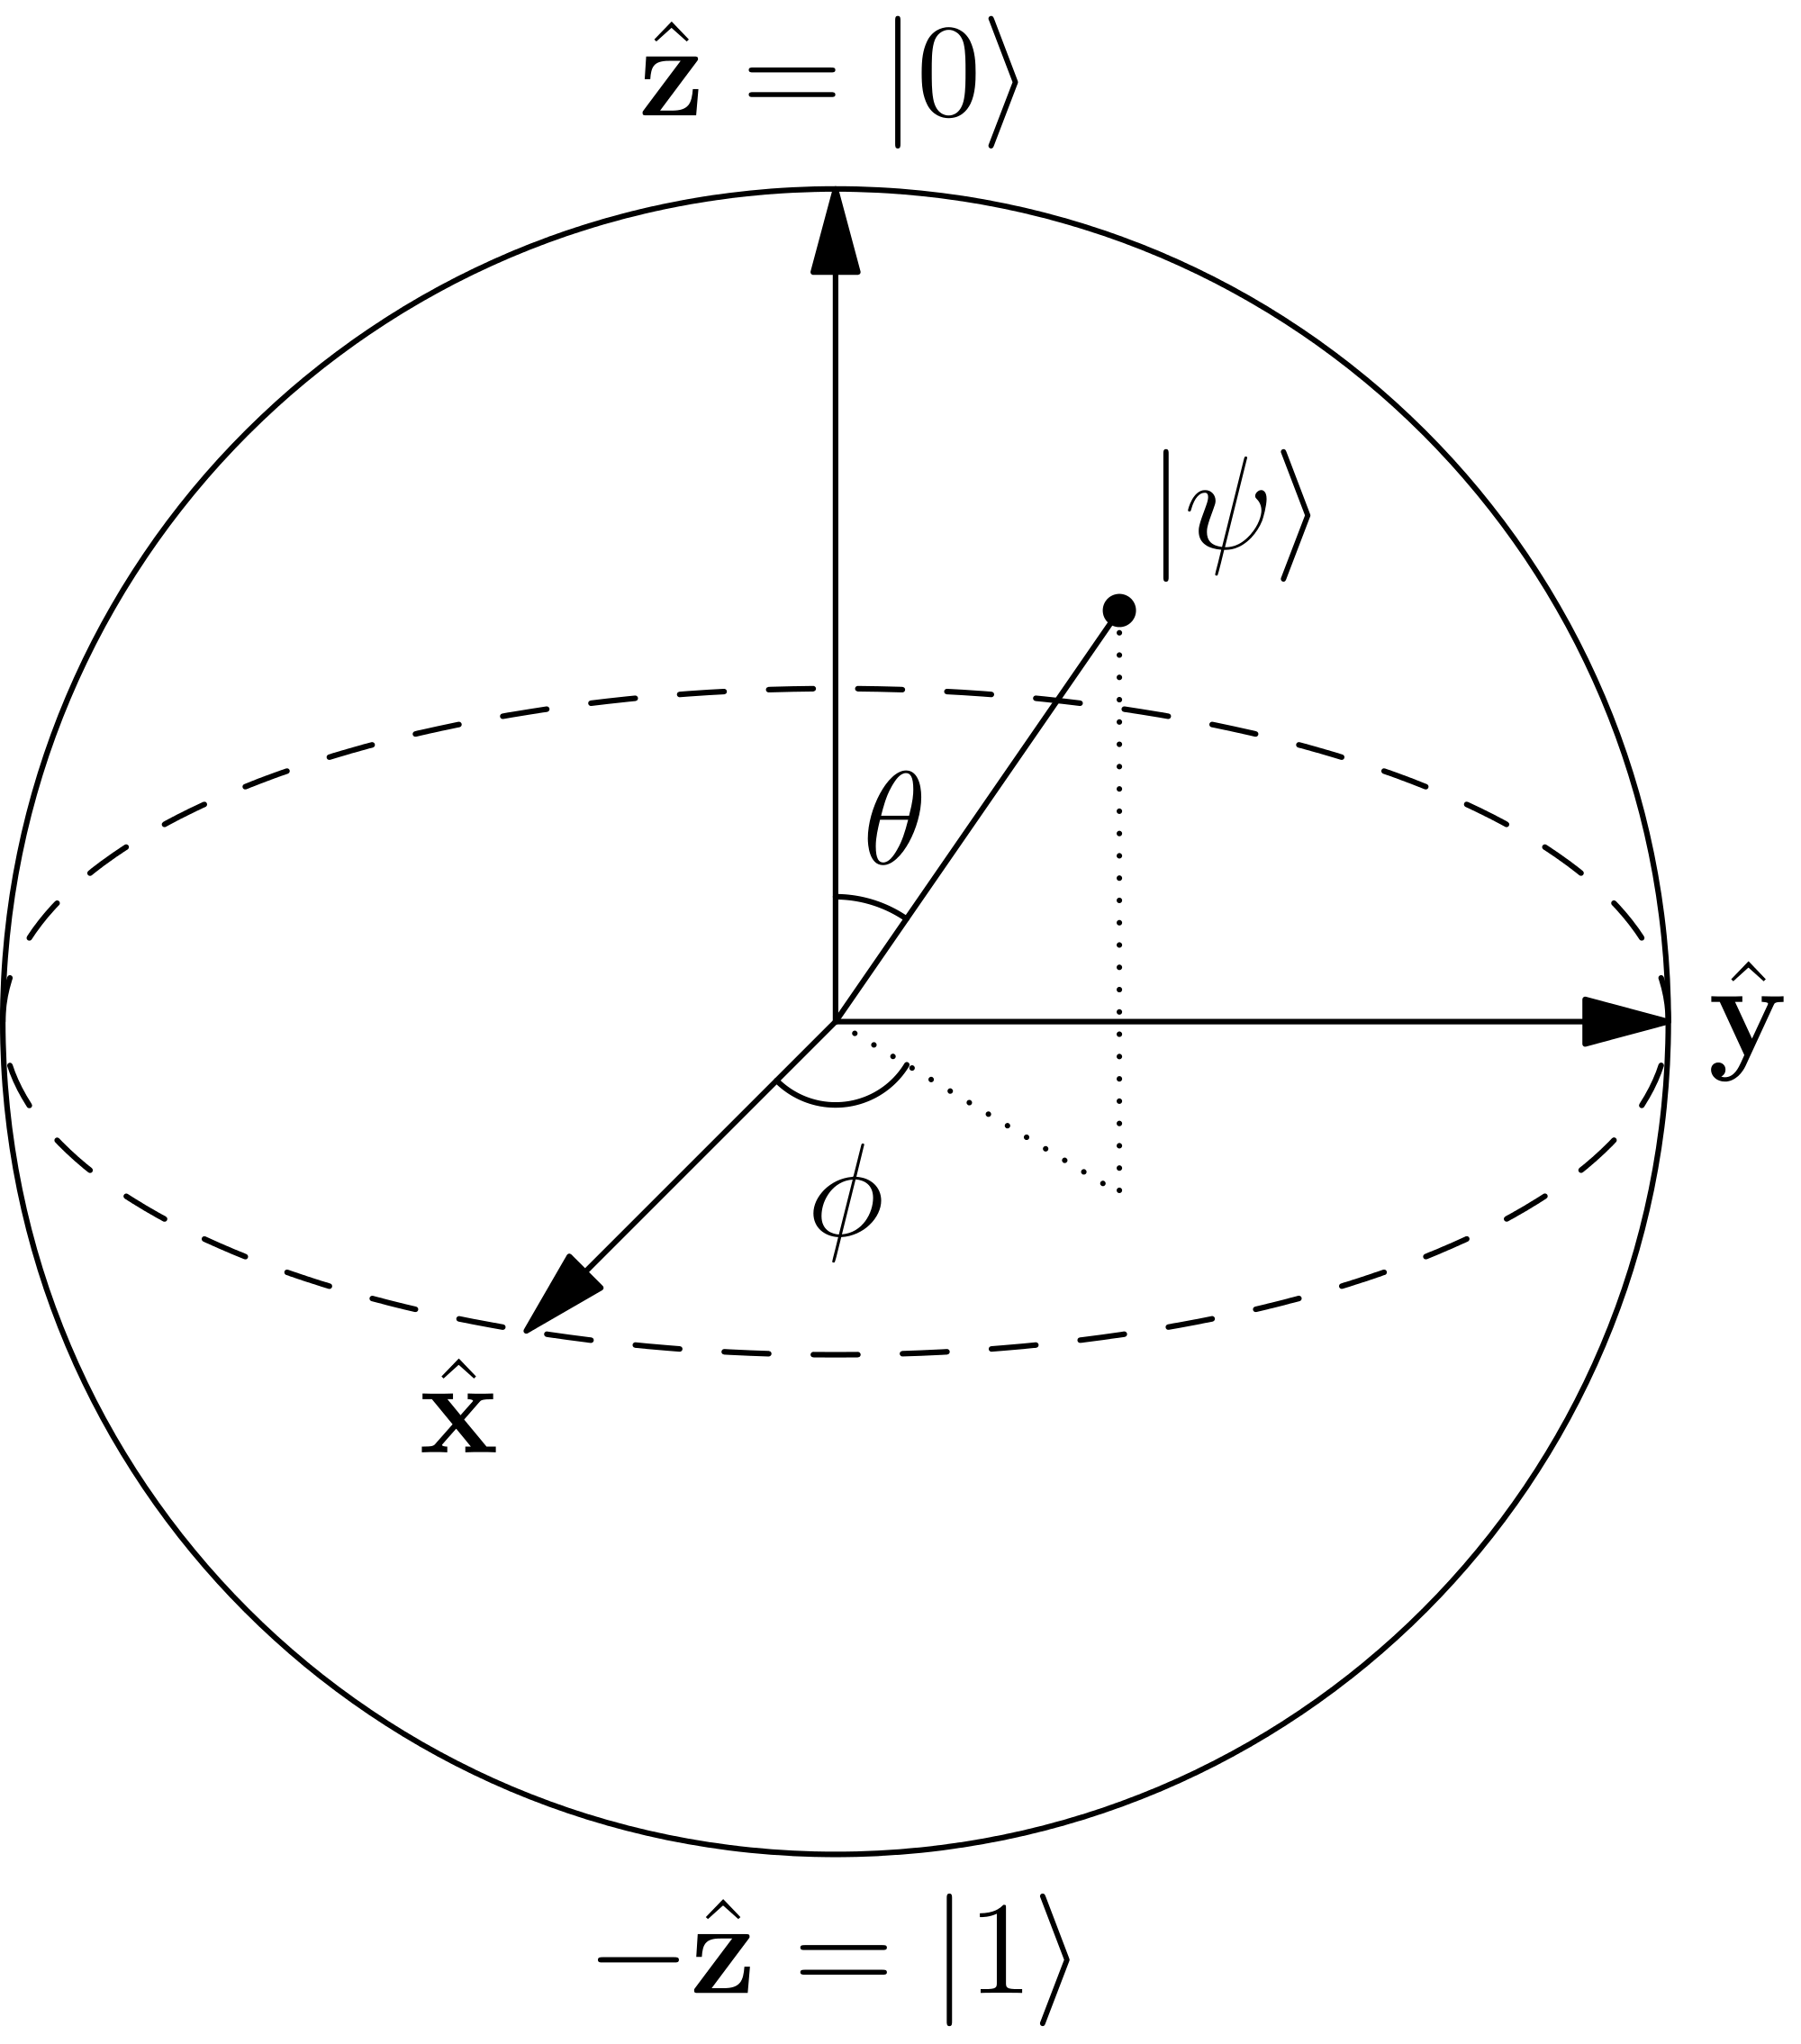
\includegraphics[width=0.8\textwidth]{blochsphere.png}
       \captionsetup{justification=raggedright, singlelinecheck=false}
       \captionof{figure}{\footnotesize{Arbitrary two-dimensional qubit $\ket{\psi}$ visualized on the Bloch sphere\textsuperscript{1}} }
\end{minipage}%%%%%
\begin{minipage}[c][][b]{.5\textwidth}
Most general form of a 2-D qubit:
\begin{equation}
\label{equ: blochqubit}
\ket{q} = \alpha \ket{0} + \beta \ket{1}
\end{equation}
where $\alpha,\beta \in \mathbb{C}$.\\
\\
Can also be visualized in spherical polar coords on the unit or Bloch sphere as follows: 

\begin{equation}
\label{equ: blochqubit}
\ket{q} = \cos\frac{\theta}{2} \ket{0} + e^{i \phi} \sin\frac{\theta}{2} \ket{1}
\end{equation}
where $0 \leq \theta \leq \pi$ and $0 \leq \phi \leq 2\pi$
\null
\par\xdef\tpd{\the\prevdepth}
\end{minipage}


\end{frame}
}

{
\setbeamertemplate{frame footer}{\tiny{\textsuperscript{1}IBM. (2016). What is big data? https://www-01.ibm.com/software/data/bigdata/what-is-big
-data.html. (Accessed: 2016-09-08) \newline
\textsuperscript{2}Bekkerman, R., Bilenko, M., \& Langford, J. (2011). Scaling up machine learning: Parallel and distributed
approaches. Cambridge University Press.}}
\begin{frame}[fragile]{Machine Learning}
   
\begin{itemize}
	\item Approximately 2.5 quintillion (${10}^{18}$) bytes of digital data are created every day\textsuperscript{1}
	\item Need for advanced algorithms that can make sense of data content, retrieve patterns and reveal correlations $\rightarrow$ Machine learning (ML) 
	\item ML algorithms often involve
	\begin{itemize}
	\item solving large systems of linear equations
	\item inverting large matrices
	\item distance computations
	\end{itemize}
	\item Performing these computations on large data
sets gets increasingly difficult\textsuperscript{2}

%when i.e. $\mathcal{O}(input size)$ or $\mathcal{O}(input size^{k})$ for some constant k\textsuperscript{2}
%essentially manipulations on big vectors and matrices

\end{itemize}

\end{frame}
}

{
\setbeamertemplate{frame footer}{}
\begin{frame}[fragile]{Machine Learning}
   
Machine learning can be subdivided into three major fields.

\metroset{block=fill}

\begin{alertblock}{Supervised ML}
- Based on \emph{input} and \emph{output} data\\
\centering{
"I know how to classify this data but I need the algorithm to do the computations for me."}
\end{alertblock}

\begin{exampleblock}{Unsupervised ML}
- Based on \emph{input} data only\\
\centering{
"I have no clue how to classify this data, can the algorithm create a classifier for me?"}
\end{exampleblock}

\begin{block}{Reinforcement learning}
- Based on \emph{input} data only\\
\centering{
"I have no clue how to classify this data, can the algorithm classify this data and I'll give it a reward if it's correct or I'll punish it if it's not."}
\end{block}

\end{frame}
}

{
\setbeamertemplate{frame footer}{}
\begin{frame}[fragile]{Machine Learning}
   
Machine learning can be subdivided into three major fields.$\mathcal{O}(input size)$

\metroset{block=fill}

\begin{alertblock}{Supervised ML}
- Based on \emph{input} and \emph{output} data\\
\centering{
"I know how to classify this data but I need the algorithm to do the computations for me."}
\end{alertblock}

\begin{exampleblock}{\textcolor{gray}{Unsupervised ML}}
\color{gray}
- Based on \emph{input} data only\\
\centering{
"I have no clue how to classify this data, can the algorithm create a classifier for me?"}
\end{exampleblock}

\begin{block}{\textcolor{gray}{Reinforcement learning}}
\color{gray}
- Based on \emph{input} data only\\
\centering{
"I have no clue how to classify this data, can the algorithm classify this data and I'll give it a reward if it's correct or I'll punish it if it's not."}
\end{block}

\end{frame}
}

{
\setbeamertemplate{frame footer}{References go here}
\begin{frame}[fragile]{Quantum Machine Learning}

Some general info about QML. How can quantum computing aid classical machine learning?

\end{frame}
}

{
\setbeamertemplate{frame footer}{References go here}
\begin{frame}[fragile]{Experimental realizations so far}


Until now there have been only few experimental verifications of QML algorithms that establish proof-
of-concept. Li, Liu, Xu, and Du (2015) successfully distinguished a handwritten six from a nine using a
quantum support vector machine on a four-qubit nuclear magnetic resonance test bench. In addition, Cai
et al. (2015) were first to experimentally demonstrate quantum machine learning on a photonic QC and
showed that the distance between two vectors and their inner product can indeed be computed quantum
mechanically. Lastly, Ristè et al. (2015) solved a learning parity problem with five superconducting qubits
and found that a quantum advantage can already be observed in non error-corrected systems.


%Explain the experimental results that have been shown so far. Outline problems with non-error corrected qubits, gate times and small qubit numbers.

%> only proof-of-concept so far
%little is known about full procedure from crude data to final classification

\end{frame}
}

{
\setbeamertemplate{frame footer}{\tiny{\textsuperscript{1}Reprinted from GitHub, Burton de Wilde, Retrieved September 13, 2016, from http://bdewilde.github.io/blog/
blogger/2012/10/26/classification-of-hand-written-digits-3/. Copyright 2012 by Burton de Wilde. Reprinted with
permission.}}
\begin{frame}[fragile]{Classical k-nearest neighbour}
 
 \begin{minipage}[t]{.5\textwidth}
      
Some description goes here.
\end{minipage}%%%%%
\begin{minipage}[c]{.5\textwidth}
%\centering
       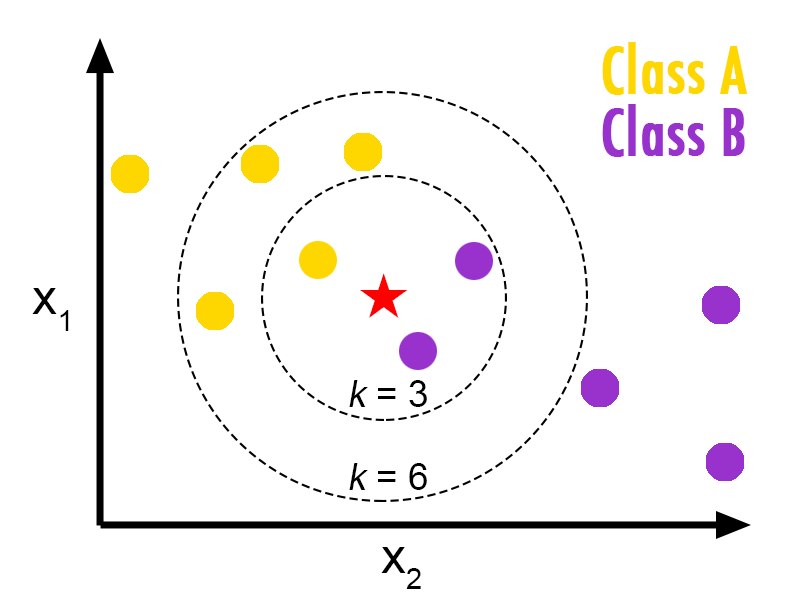
\includegraphics[width=\textwidth]{knn-concept.png}
       \captionsetup{justification=raggedright, singlelinecheck=false}
      \captionof{figure}{\footnotesize{Visualization of a kNN classifier\footnotemark[1]}}

\end{minipage}

 
\end{frame}
}

{
\setbeamertemplate{frame footer}{}
\begin{frame}[fragile]{Quantum k-nearest neighbour}
 
Two different algorithms with respect to initial state preparation:

\begin{alertblock}{Data encoded into qubits}
%speed-up not very clear since the \# of qubits increases linearly with the \# of classical bits
k-dimensional probability vector requires $4k$ classical bits which are encoded one-to-one into $4k$ qubits, e.g.\\
\vspace{2mm}
$\begin{pmatrix}
 \textcolor{blue}{0.6} \\ 
 \textcolor{orange}{0.4}
 \end{pmatrix}*10 \rightarrow \begin{pmatrix}
 \textcolor{blue}{6} \\ 
 \textcolor{orange}{4}
 \end{pmatrix} \rightarrow \begin{pmatrix}
 \textcolor{blue}{0110} \\ 
 \textcolor{orange}{0100}
 \end{pmatrix} \rightarrow n=\textcolor{blue}{0110}\textcolor{orange}{0100} \rightarrow \ket{n} = \ket{\textcolor{blue}{0110}\textcolor{orange}{0100}}$\\
%\textbf{Only slight speed up possible}
\end{alertblock}
\vspace{3mm}
\begin{alertblock}{\textcolor{gray}{Data encoded into amplitudes}}
\textcolor{gray}{k-dimensional probability vector is encoded into $log_{2}(k)$ qubits, e.g.\\ 
\vspace{2mm}
$\begin{pmatrix}
 0.6 \\ 
 0.4
 \end{pmatrix} \quad \rightarrow \quad \ket{n} = \sqrt{0.6}\ket{0}+\sqrt{0.4}\ket{1}$\\
%\textbf{Possibility of exponential speed up}
}
\end{alertblock}

\end{frame}
}

{
\setbeamertemplate{frame footer}{}
\begin{frame}[fragile]{Quantum k-nearest neighbour}
 
Two different algorithms with respect to initial state preparation:

\begin{alertblock}{\textcolor{gray}{Data encoded into qubits}}
%speed-up not very clear since the \# of qubits increases linearly with the \# of classical bits
\textcolor{gray}{k-dimensional probability vector requires $4k$ classical bits which are encoded one-to-one into $4k$ qubits, e.g.\\
\vspace{2mm}
$\begin{pmatrix}
 0.6 \\ 
 0.4
 \end{pmatrix}*10 \rightarrow \begin{pmatrix}
 6 \\ 
 4
 \end{pmatrix} \rightarrow \begin{pmatrix}
 0110 \\ 
 0100
 \end{pmatrix} \rightarrow n=01100100 \rightarrow \ket{n} = \ket{01100100}$\\
%\textbf{Only slight speed up possible}
}
\end{alertblock}  
\vspace{3mm}
\begin{alertblock}{Data encoded into amplitudes}
k-dimensional probability vector is encoded into $log_{2}(k)$ qubits, e.g.\\ 
\vspace{2mm}
$\begin{pmatrix}
 \textcolor{blue}{0.6} \\ 
 \textcolor{orange}{0.4}
 \end{pmatrix} \quad \rightarrow \quad \ket{n} = \sqrt{\textcolor{blue}{0.6}}\ket{0}+\sqrt{\textcolor{orange}{0.4}}\ket{1}$\\
%\textbf{Possibility of exponential speed up}
\end{alertblock}


\end{frame}
}


\section{Amplitude-based kNN algorithm}
{
\setbeamertemplate{frame footer}{\vspace{-2mm}\tiny{Maria Schuld (2016), unpublished}}
\begin{frame}{The algorithm}

\begin{equation}
\frac{1}{\sqrt{2M}}\sum_{m=1}^{M} (\ket{0}\ket{\Psi_{\tilde{x}}}+\ket{1}\ket{\Psi_{x^{m}}})\ket{y^{m}}\ket{m}
\end{equation}
where
\begin{equation}
\ket{\Psi_{\tilde{x}}} = \sum_{i=1}^{N} \tilde{x}_i\ket{i} \quad \quad
\ket{\Psi_{x^{m}}} = \sum_{i=1}^{N} x_i^m \ket{i}
\end{equation}

\begin{equation}
\frac{1}{2\sqrt{M}}\sum_{m=1}^{M} (\ket{0}[\ket{\Psi_{\tilde{x}}}+\ket{\Psi_{x^{m}}}]+\ket{1}[\ket{\Psi_{\tilde{x}}}-\ket{\Psi_{x^{m}}}])\ket{y^{m}}\ket{m}
\end{equation}
After successful conditional measurement, the state is proportional to
\begin{equation}
\frac{1}{2\sqrt{M}}\sum_{m=1}^{M} \sum_{i=1}^{N} (\tilde{x}_i+x_i^m)\ket{0}\ket{i}\ket{y^{m}}\ket{m}
\end{equation}
	
	\metroset{block=fill}
	\begin{alertblock}{Algorithmic complexity}
	\centering
	$\mathcal{O}(\frac{1}{p_{acc}})$ where $p_{acc}$ is the probability of measuring ancilla in the $\ket{0}$ state
	\end{alertblock}
\end{frame}
}

{
\setbeamertemplate{frame footer}{}
\begin{frame}{Simple binary classification case}

\begin{minipage}[c]{.4\textwidth}
		%\centering
		\hspace{-7mm}
       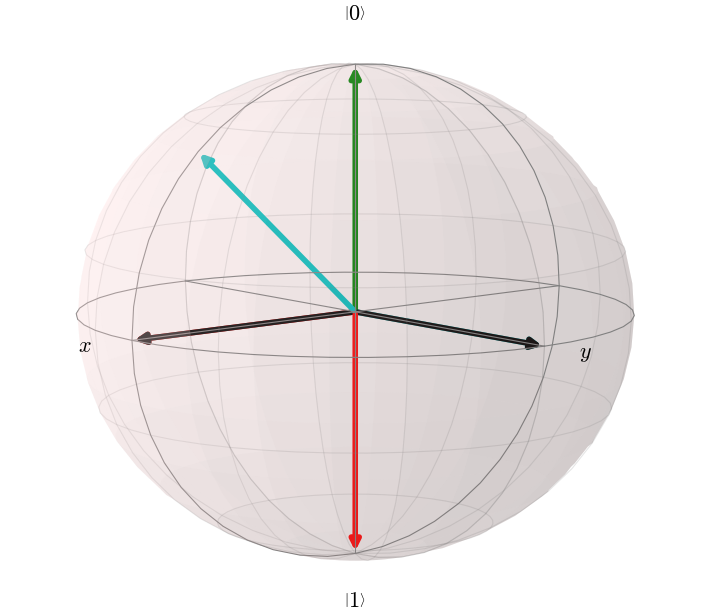
\includegraphics[width=\textwidth]{bloch3over4.png}
       \captionsetup{justification=raggedright, singlelinecheck=false}
       \captionof{figure}{\footnotesize{Simple binary classification problem of a quantum state} }
\end{minipage}%%%%
\begin{minipage}[c][][b]{.6\textwidth}
\scriptsize{
\begin{equation}
\frac{1}{\sqrt{2M}}\sum_{m=1}^{M} (\ket{0}\ket{\Psi_{\tilde{x}}}+\ket{1}\ket{\Psi_{x^{m}}})\ket{y^{m}}\ket{m}
\end{equation}
where
\begin{equation}
\ket{\Psi_{\tilde{x}}} = \sum_{i=1}^{N} \tilde{x}_i\ket{i} \quad \quad
\ket{\Psi_{x^{m}}} = \sum_{i=1}^{N} x_i^m \ket{i}
\end{equation}}
Procedure to load the input vector $\tilde{x}$:
\begin{equation}
\ket{\Psi_0} = \frac{1}{2}\sum_{m=1}^{2} (\ket{0}\ket{0}+\ket{1}\ket{0})\ket{y^{m}}\ket{m}
\end{equation}
Apply controlled rotation $_0^1CR_y(\frac{\pi}{4})$ s.t.
\begin{equation}
_0^1CR_y(\frac{\pi}{4})\ket{\Psi_0} = \ket{\Psi_1} = \frac{1}{2}\sum_{m=1}^{2} (\ket{0}\ket{0}+\ket{1}\ket{\Psi_{\tilde{x}}})\ket{y^{m}}\ket{m}
\end{equation}
Flip the ancilla qubit in the first register
\begin{equation}
(X\otimes\mathds{1}\otimes\mathds{1}\otimes\mathds{1})\ket{\Psi_1} = \ket{\Psi_2} = \frac{1}{2}\sum_{m=1}^{2} (\ket{0}\ket{\Psi_{\tilde{x}}}+\ket{1}\ket{0})\ket{y^{m}}\ket{m}
\end{equation}
\null
\par\xdef\tpd{\the\prevdepth}
\end{minipage}

	%\metroset{block=fill}
	%\begin{alertblock}{Algorithmic complexity}
	%\centering
	%$\mathcal{O}(\frac{1}{p_{acc}})$
	%\end{alertblock}

\end{frame}
}

{
\setbeamertemplate{frame footer}{}
\begin{frame}{Implementation with IBM's quantum computer}

\begin{minipage}[c]{.4\textwidth}
Minipage 1
\end{minipage}%%%%
\begin{minipage}[c][][b]{.6\textwidth}
Minipage 2
\end{minipage}


\end{frame}
}

{
\setbeamertemplate{frame footer}{\tiny{\textsuperscript{1}Nielsen, M. A., \& Chuang, I. L. (2010). Quantum computation and quantum information. Cambridge University Press.\newline \textsuperscript{2}Jat, R. N., \& Ruhela, D. S. (2011). Comparative study of complexity of algorithms for iterative solution of non-linear equations. Journal of International Academy Of Physical Sciences, 15(4).}}
\begin{frame}{Controlled U gate}

\begin{minipage}[t]{.4\textwidth}
	%\vspace{-20mm}
	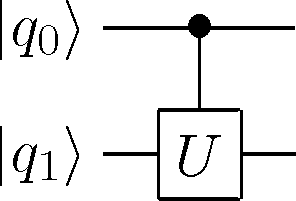
\includegraphics[height=0.5\textwidth]{controlledU.png}
       \captionsetup{justification=raggedright, singlelinecheck=false}
       \captionof{figure}{\footnotesize{Controlled U-gate} }
\end{minipage}%%%%%
\begin{minipage}[t]{.6\textwidth}
%\vspace{-20mm}
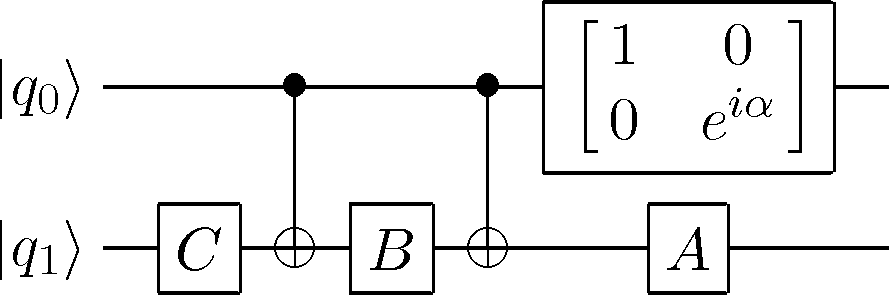
\includegraphics[width=1\textwidth]{controlledUdecomposition.png}
       \captionsetup{justification=raggedright, singlelinecheck=false}
       \captionof{figure}{\footnotesize{Decomposition of a controlled U-gate\textsuperscript{1}} }
\end{minipage}

Choose A,B,C and $\alpha$ s.t.
\begin{equation}
e^{i\alpha}*A*X*B*X*C = U \quad and \quad A*B*C = \mathds{1}
\end{equation}
Need to solve the following equation\textsuperscript{1}
\begin{equation}
U = \begin{pmatrix}
 e^{i(\alpha-\frac{\beta}{2}-\frac{\delta}{2})}\cos{\frac{\gamma}{2}} & -e^{i(\alpha-\frac{\beta}{2}+\frac{\delta}{2})}\sin{\frac{\gamma}{2}} \\ 
e^{i(\alpha+\frac{\beta}{2}-\frac{\delta}{2})}\sin{\frac{\gamma}{2}} & e^{i(\alpha+\frac{\beta}{2}+\frac{\delta}{2})}\cos{\frac{\gamma}{2}}
 \end{pmatrix}
\end{equation}

%calculating a root of a function f(x) with n-digit precision, provided that a good initial approximation is known, is O((\log n) F(n)) where F(n) is the cost of calculating f(x)/f'(x)\, with n-digit precision.

	\metroset{block=fill}
	\begin{alertblock}{Algorithmic complexity}
	$\mathcal{O}(\frac{1}{p_{acc}})+\mathcal{O}(k)$ where $k$ is number of root finding iterations\textsuperscript{2}
	\end{alertblock}
\end{frame}

}

{
\setbeamertemplate{frame footer}{\tiny{\textsuperscript{1}Dawson, C. M., \& Nielsen, M. A. (2005). The Solovay-Kitaev algorithm. arXiv preprint quant-ph/0505030.}}
\begin{frame}{Problems with universal gate sets}

In our case we need to find A, B, C and $\alpha$ for $_0^1CR_y(\frac{\pi}{4})$:

Using a root finding algorithm for non-linear equations we find:

\begin{equation}
\alpha =  \pi; \quad 
\beta = 2\pi;\quad 
\delta = \frac{7}{8}\pi;\quad 
\gamma = 0
\end{equation}
Then,
\begin{align}
A \quad= \quad R_z(\beta)R_y(\frac{\gamma}{2})\quad =& \quad R_z(2\pi) \quad = \quad \textcolor{green}{XZXZ} \\
B\quad =\quad R_y(-\frac{\gamma}{2})R_z(-\frac{\delta+\beta}{2})\quad =& \quad R_z(-\frac{23}{16}\pi) \quad= \quad \textcolor{red}{???}  \\
C \quad=\quad R_z(\frac{\delta-\beta}{2})\quad =& \quad R_z(-\frac{9}{16}\pi) \quad= \quad \textcolor{red}{???} \\
\begin{pmatrix} 1&0\cr0&e^{i\alpha} \end{pmatrix}\quad=& \quad \begin{pmatrix} 1&0\cr0&e^{i\pi} \end{pmatrix}\quad= \quad \textcolor{green}{Z}
\end{align}

\end{frame}
}

{
\setbeamertemplate{frame footer}{\tiny{\textsuperscript{1}Dawson, C. M., \& Nielsen, M. A. (2005). The Solovay-Kitaev algorithm. arXiv preprint quant-ph/0505030.}}
\begin{frame}{The Solovay-Kitaev theorem}

The Solovay-Kitaev theorem guarantees that given a set of single-qubit quantum gates which generates a dense subset of $SU(2)$, then that set is guaranteed to fill $SU(2)$ quickly.\textsuperscript{1}
 
$\rightarrow$ \textcolor{green}{\textbf{Hence, given any universal gate set it is possible to obtain good approximations to any desired gate.}}

$\rightarrow$ \textcolor{red}{\textbf{But needs to be computed classically!}}
\vspace{16mm}
\metroset{block=fill}
	\begin{alertblock}{Algorithmic complexity}
	$\mathcal{O}(\frac{1}{p_{acc}})+\mathcal{O}(k)+\mathcal{O}(m*log^{2.71}(\frac{m}{\epsilon}))$ for $\epsilon$-approximations of $m$ gates\textsuperscript{1}
	\end{alertblock}
\end{frame}
}

{
\setbeamertemplate{frame footer}{}
\begin{frame}{The Solovay-Kitaev algorithm}

What is fowler distance?

\begin{figure}
    \begin{tikzpicture}
\begin{axis}[xlabel={Gate count},ylabel={Fowler distance [$d(U,U_{approx})$]}]

% Graph column 2 versus column 0
\addplot table[x index=1,y index=0,col sep=comma] {datax.dat};
\addlegendentry{$R_z(-\frac{9}{16}\pi)$}% y index+1 since humans count from 1

% Graph column 1 versus column 0    
\addplot table[x index=5,y index=4,col sep=comma] {datax.dat};
\addlegendentry{$R_z(-\frac{23}{16}\pi)$}

\end{axis}
\end{tikzpicture}
  \end{figure}

\end{frame}
}

{
\setbeamertemplate{frame footer}{}
\begin{frame}{The Solovay-Kitaev algorithm}

%SK needs to be implemented for each gate that is not element of the universal gate set:
%\begin{align}
%R_z(-\frac{23}{16}\pi) \quad \rightarrow& \quad  %\\
%R_z(-\frac{9}{16}\pi) \quad \rightarrow& \quad 121 gates \quad (d(U,U_{approx}) = 0.04389)
%\end{align}

IBM's quantum computer needs \textbf{130ns for single-qubit gates} and \textbf{500ns for CNOT gates.}

Qubit decoherence times:

\SI{49.5}{\micro\second} $\leq T1 \leq$ \SI{85.3}{\micro\second}\\
\SI{56.0}{\micro\second} $\leq T2 \leq$ \SI{139.7}{\micro\second}
\vspace{6mm}
\begin{table}
    \begin{tabular}{c| c |c |c}
      \toprule
      Approx. Gate & Distance & Gate count & Execution time\\
      \midrule
      $R_z(-\frac{9}{16}\pi)$ & 0.04389 & 121 & \textcolor{green}{\SI{15.7}{\micro\second}}\\
       & 0.02823 & 3,622 & \textcolor{red}{\SI{470.9}{\micro\second}}\\
       & 0.004698 & 20,496 & \textcolor{red}{\SI{2664.5}{\micro\second}}\\
       %& 14,160,467 & 20,116,842 & 20,116,842\\
      \bottomrule
    \end{tabular}
    \caption{SK algorithm results}
  \end{table}

\end{frame}
}

{
\setbeamertemplate{frame footer}{}
\begin{frame}{Liqui$\ket{}$ simulations}
	
Show that the simple binary classification problem works in Liquid since we can directly implement the controlled $R_z$ rotations

%Run the command mono Liquid.exe "__BinaryAmplitudeKNN(10000)" in a terminal

Could you also show what happens if I use approximated gate sequences?
	
\end{frame}
}

{
\setbeamertemplate{frame footer}{}
\begin{frame}{Liqui$\ket{}$ simulations: Taking it further}

\begin{figure}
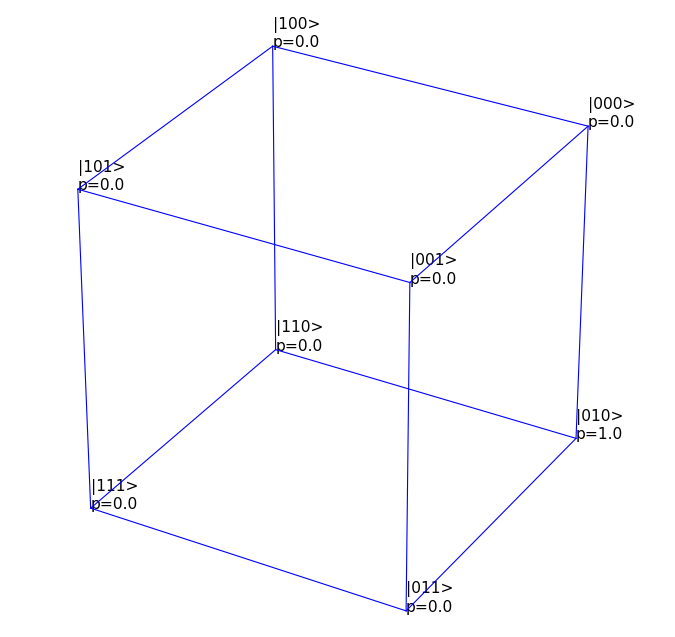
\includegraphics[scale=0.35]{cube_notdiffused.png}
       \caption{\footnotesize{Representation of hamming distance on 3D cube} }
\end{figure}
\end{frame}
}

{
\setbeamertemplate{frame footer}{}
\begin{frame}{Liqui$\ket{}$ simulations: Taking it further}

Applying the following matrix
\begin{equation}
\begin{pmatrix}
 \sqrt{\delta} & 1-\sqrt{\delta} \\ 
 1-\sqrt{\delta} & -\sqrt{\delta}
 \end{pmatrix}
\end{equation}
to all qubits in the data register leads to a gaussian distribution over the "Hamming distance" cube:

\begin{figure}
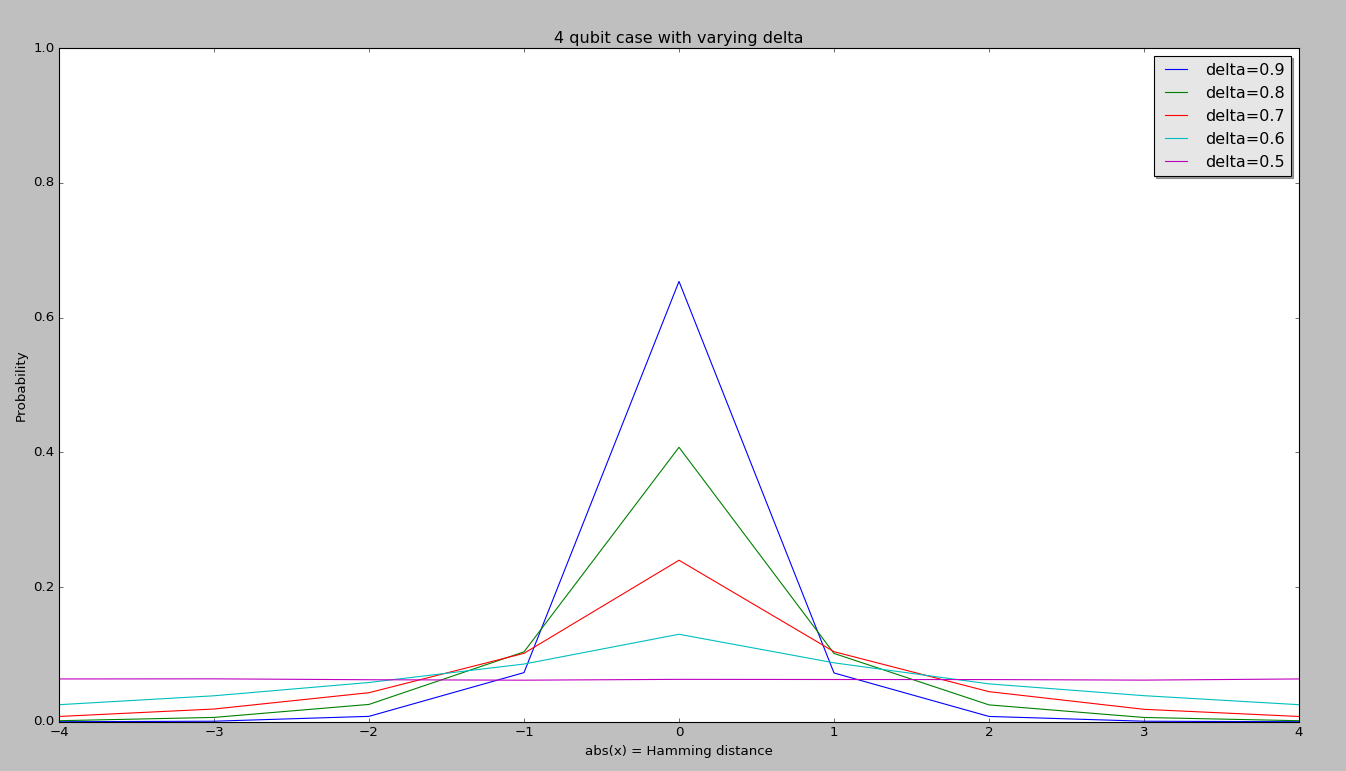
\includegraphics[scale=0.2]{4qubitdiffusion.png}
       \caption{\footnotesize{Gaussian diffusion of a quantum state} }
\end{figure}

\end{frame}
}

{
\setbeamertemplate{frame footer}{}
\begin{frame}{Liqui$\ket{}$ simulations: Taking it further}

\begin{figure}
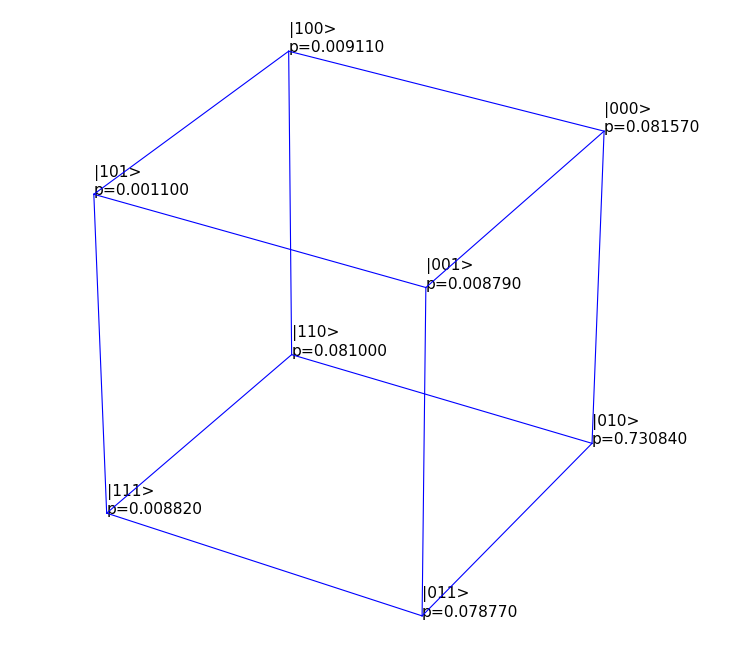
\includegraphics[scale=0.33]{cube_diffused.png}
       \caption{\footnotesize{Representation of gaussian diffusion on 3D cube} }
\end{figure}
\end{frame}
}

{
\setbeamertemplate{frame footer}{}
\begin{frame}{Liqui$\ket{}$ simulations: Taking it further}

\begin{figure}
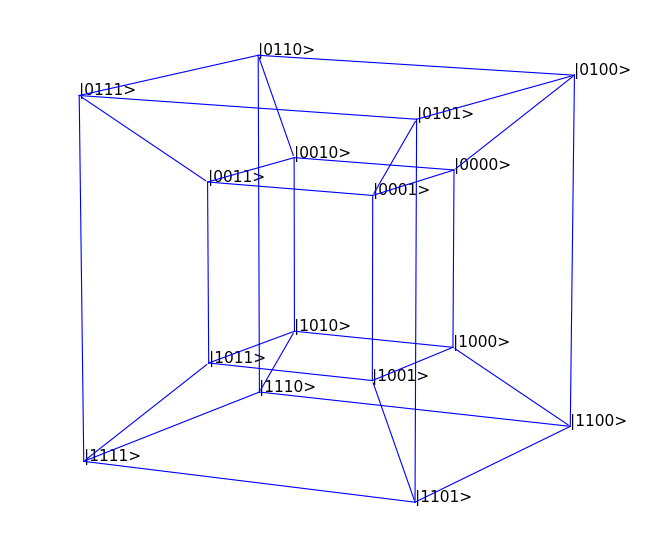
\includegraphics[scale=0.33]{4d_hypercube.png}
       \caption{\footnotesize{Representation of gaussian diffusion on 3D cube} }
\end{figure}
\end{frame}
}


\section{Conclusion}

\begin{frame}{Summary}

sefsefesfsefsef
\end{frame}

\begin{frame}{References}
  Some references to showcase [allowframebreaks] \cite{knuth92,ConcreteMath,Simpson,Er01,greenwade93}
\end{frame}

\begin{frame}[standout]
  Questions?
\end{frame}


\appendix

\begin{frame}[fragile]{Backup slide I}
fefesfesfesfefesf
\end{frame}

\begin{frame}[allowframebreaks]{Backup slide II}

  \bibliography{demo}
  \bibliographystyle{abbrv}

\end{frame}

\section{Qubit-based kNN quantum algorithm}

{
\setbeamertemplate{frame footer}{References go here}
\begin{frame}[fragile]{Typography}
      \begin{verbatim}The theme provides sensible defaults to
\emph{emphasize} text, \alert{accent} parts
or show \textbf{bold} results.\end{verbatim}

  \begin{center}becomes\end{center}

  The theme provides sensible defaults to \emph{emphasize} text,
  \alert{accent} parts or show \textbf{bold} results.
\end{frame}
}

{
\setbeamertemplate{frame footer}{References go here}
\begin{frame}{Font feature test}
  \begin{itemize}
    \item Regular
    \item \textit{Italic}
    \item \textsc{SmallCaps}
    \item \textbf{Bold}
    \item \textbf{\textit{Bold Italic}}
    \item \textbf{\textsc{Bold SmallCaps}}
    \item \texttt{Monospace}
    \item \texttt{\textit{Monospace Italic}}
    \item \texttt{\textbf{Monospace Bold}}
    \item \texttt{\textbf{\textit{Monospace Bold Italic}}}
  \end{itemize}
\end{frame}
}

\begin{frame}{Lists}
  \begin{columns}[T,onlytextwidth]
    \column{0.33\textwidth}
      Items
      \begin{itemize}
        \item Milk \item Eggs \item Potatos
      \end{itemize}

    \column{0.33\textwidth}
      Enumerations
      \begin{enumerate}
        \item First, \item Second and \item Last.
      \end{enumerate}

    \column{0.33\textwidth}
      Descriptions
      \begin{description}
        \item[PowerPoint] Meeh. \item[Beamer] Yeeeha.
      \end{description}
  \end{columns}
\end{frame}
\begin{frame}{Animation}
  \begin{itemize}[<+- | alert@+>]
    \item \alert<4>{This is\only<4>{ really} important}
    \item Now this
    \item And now this
  \end{itemize}
\end{frame}
\begin{frame}{Figures}
  \begin{figure}
    \newcounter{density}
    \setcounter{density}{20}
    \begin{tikzpicture}
      \def\couleur{alerted text.fg}
      \path[coordinate] (0,0)  coordinate(A)
                  ++( 90:5cm) coordinate(B)
                  ++(0:5cm) coordinate(C)
                  ++(-90:5cm) coordinate(D);
      \draw[fill=\couleur!\thedensity] (A) -- (B) -- (C) --(D) -- cycle;
      \foreach \x in {1,...,40}{%
          \pgfmathsetcounter{density}{\thedensity+20}
          \setcounter{density}{\thedensity}
          \path[coordinate] coordinate(X) at (A){};
          \path[coordinate] (A) -- (B) coordinate[pos=.10](A)
                              -- (C) coordinate[pos=.10](B)
                              -- (D) coordinate[pos=.10](C)
                              -- (X) coordinate[pos=.10](D);
          \draw[fill=\couleur!\thedensity] (A)--(B)--(C)-- (D) -- cycle;
      }
    \end{tikzpicture}
    \caption{Rotated square from
    \href{http://www.texample.net/tikz/examples/rotated-polygons/}{texample.net}.}
  \end{figure}
\end{frame}
\begin{frame}{Tables}
  \begin{table}
    \caption{Largest cities in the world (source: Wikipedia)}
    \begin{tabular}{lr}
      \toprule
      City & Population\\
      \midrule
      Mexico City & 20,116,842\\
      Shanghai & 19,210,000\\
      Peking & 15,796,450\\
      Istanbul & 14,160,467\\
      \bottomrule
    \end{tabular}
  \end{table}
\end{frame}
\begin{frame}{Blocks}
  Three different block environments are pre-defined and may be styled with an
  optional background color.

  \begin{columns}[T,onlytextwidth]
    \column{0.5\textwidth}
      \begin{block}{Default}
        Block content.
      \end{block}

      \begin{alertblock}{Alert}
        Block content.
      \end{alertblock}

      \begin{exampleblock}{Example}
        Block content.
      \end{exampleblock}

    \column{0.5\textwidth}

      \metroset{block=fill}

      \begin{block}{Default}
        Block content.
      \end{block}

      \begin{alertblock}{Alert}
        Block content.
      \end{alertblock}

      \begin{exampleblock}{Example}
        Block content.
      \end{exampleblock}

  \end{columns}
\end{frame}
\begin{frame}{Math}
  \begin{equation*}
    e = \lim_{n\to \infty} \left(1 + \frac{1}{n}\right)^n
  \end{equation*}
\end{frame}
\begin{frame}{Line plots}
  \begin{figure}
    \begin{tikzpicture}
      \begin{axis}[
        mlineplot,
        width=0.9\textwidth,
        height=6cm,
      ]

        \addplot {sin(deg(x))};
        \addplot+[samples=100] {sin(deg(2*x))};

      \end{axis}
    \end{tikzpicture}
  \end{figure}
\end{frame}
\begin{frame}{Bar charts}
  \begin{figure}
    \begin{tikzpicture}
      \begin{axis}[
        mbarplot,
        xlabel={Foo},
        ylabel={Bar},
        width=0.9\textwidth,
        height=6cm,
      ]

      \addplot plot coordinates {(1, 20) (2, 25) (3, 22.4) (4, 12.4)};
      \addplot plot coordinates {(1, 18) (2, 24) (3, 23.5) (4, 13.2)};
      \addplot plot coordinates {(1, 10) (2, 19) (3, 25) (4, 15.2)};

      \legend{lorem, ipsum, dolor}

      \end{axis}
    \end{tikzpicture}
  \end{figure}
\end{frame}
\begin{frame}{Quotes}
  \begin{quote}
    Veni, Vidi, Vici
  \end{quote}
\end{frame}


\end{document}
